\documentclass{article}
\usepackage[utf8]{inputenc}
\usepackage[T1]{fontenc}
\usepackage[portuguese]{babel}
\usepackage{minted}
\usepackage{graphicx}
\usepackage{vmargin}
\usepackage{parskip}
\usepackage{fancyhdr}
\usepackage{titling}
\usepackage[hidelinks]{hyperref}

\graphicspath{{./images/}}

\setmarginsrb{3 cm}{2.5 cm}{3 cm}{2.5 cm}{1 cm}{1.5 cm}{1 cm}{1.5 cm}

\title{T2 - Redes de Computadores}
\author{MIEIC04\_G01}
\date{Dezembro 2018}

\pagestyle{fancy}
\fancyhf{}
\rhead{\theauthor}
\lhead{\thetitle}
\cfoot{\thepage}

\begin{document}

\begin{titlepage}
	\centering
    \vspace*{0.5 cm}
    
\includegraphics[scale = 0.5]{feup_logo.png}\\[1.0 cm]	% University Logo
    \textsc{\LARGE Faculdade de Engenharia da Universidade do Porto}\\[2.0 cm]	% University Name
	\textsc{\Large EIC0032}\\[0.5 cm]				% Course Code
	\textsc{\large Redes de Computadores}\\[0.5 cm]				% Course Name
	\rule{\linewidth}{0.2 mm} \\[0.4 cm]
	{ \huge \bfseries \thetitle}\\ 
	\rule{\linewidth}{0.2 mm} \\[1.5 cm]
	
	\begin{minipage}{0.4\textwidth}
		\begin{flushleft} \large
			\emph{Autores:}\\
            João Miguel\\
            Miguel Barraca\\
            Pedro Fernandes
        \end{flushleft}
    \end{minipage}~
    \begin{minipage}{0.4\textwidth}
        \begin{flushright} \large
            \emph{Números de estudante:} \\
            up201604241@fe.up.pt
            up201609149@fe.up.pt
            up201603846@fe.up.pt
            % Your Student Number
		\end{flushright}
\end{minipage}\\[2 cm]
	
{\large \thedate}\\[2 cm]
 
\vfill
	
\end{titlepage}

\tableofcontents
\clearpage
 
\section{Introdução}
No âmbito da Unidade Curricular Rede de Computadores (RCOM), foi-nos proposto o desenvolvimento de um projeto composto por duas partes: uma primeira que visou a criação de uma aplicação de \textit{download} e uma segunda que teve como objetivo a configuração de uma rede.  

No que diz respeito à primeira parte do trabalho, procedemos ao desenvolvimento da aplicação em linguagem de programação C, capaz de fazer o \textit{download} de ficheiros de um servidor FTP. Numa segunda fase, realizamos a configuração de uma rede e a análise de cada uma das experiências.  

Ao longo do presente relatório, pretendemos explicitar a base teórica que sustentou a elaboração deste projeto, levar a cabo uma análise do trabalho prático realizado e da aprendizagem que resultou da concretização do mesmo. 

\section{Aplicação \textit{download}}
\subsection{Arquitetura}

A aplicação tem o objetivo de fazer o \textit{download} de um ficheiro recorrendo ao protocolo
FTP (\textit{File Transfer Protocol}). Para tal, recebe como argumento um link FTP, que deve conter
os seguintes campos:

\begin{itemize}
\item Nome de utilizador
\item Palavra-passe
\item Endereço do anfitrião
\item Caminho do ficheiro
\end{itemize}

Caso os dados do utilizador não sejam fornecidos, o programa pedi-los-á posteriormente.
Após a análise do argumento, o programa cria a ligação através de duas funções cujo código 
é já fornecido:

\begin{itemize}
\item \mintinline{C}{char *getServerIp(info_t info)}
\item \mintinline{C}{int createSocketTCP(char *server_ip, int server_port)}
\end{itemize}

Em caso de conexão bem sucedida, o programa segue os seguintes passos:
\begin{enumerate}
\item Enviar \mintinline{bash}{USER} e \mintinline{bash}{PASS}
\item Entrar em modo passivo \mintinline{bash}{pasv}
\item Criar novo socket TCP
\item Enviar comando \mintinline{bash}{RETR}
\item Transferir o ficheiro
\item Terminar a conexão com \mintinline{bash}{QUIT}
\end{enumerate}

Esta estrutura é apoiada nas seguintes funções, cuja documentação pode ser encontrada nos anexos:
\begin{itemize}
\item \mintinline{C}{int sendCommand(int socketFd, char *command, char *argument)}
\item \mintinline{C}{int readServerReply(int socketFd, char *reply)}
\item \mintinline{C}{void createFile(int fd, char *filename)}
\end{itemize}

E nas seguintes estruturas:

\begin{itemize}
\item \mintinline{C}{enum state_t}
\item[] Representa o estado da leitura da resposta aos comandos enviados.
\item \mintinline{C}{enum reply_type_t}
\item[] Representa o tipo da resposta do servidor aos comandos enviados. 
\item \mintinline{C}{struct info_t}
\item[] Guarda informação fornecida no argumento do programa. 
\end{itemize}


Ao longo do programa são impressas mensagens para informar o utilizador do avanço do processo.
\subsection{Exemplo de um \textit{download} com sucesso}
Após efetuar todas as experiências, o programa foi corrido 
com o argumento \newline \textit{ftp://ftp.up.pt/pub/sage/index.html}.
O resultado é o que se pode observar nas imagens:

\begin{figure}[h]
\centering
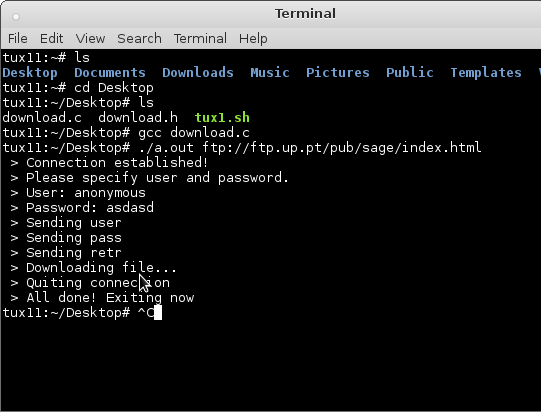
\includegraphics[width=8cm]{images/screen_dl.png}
\end{figure}

\begin{figure}[H]
\centering
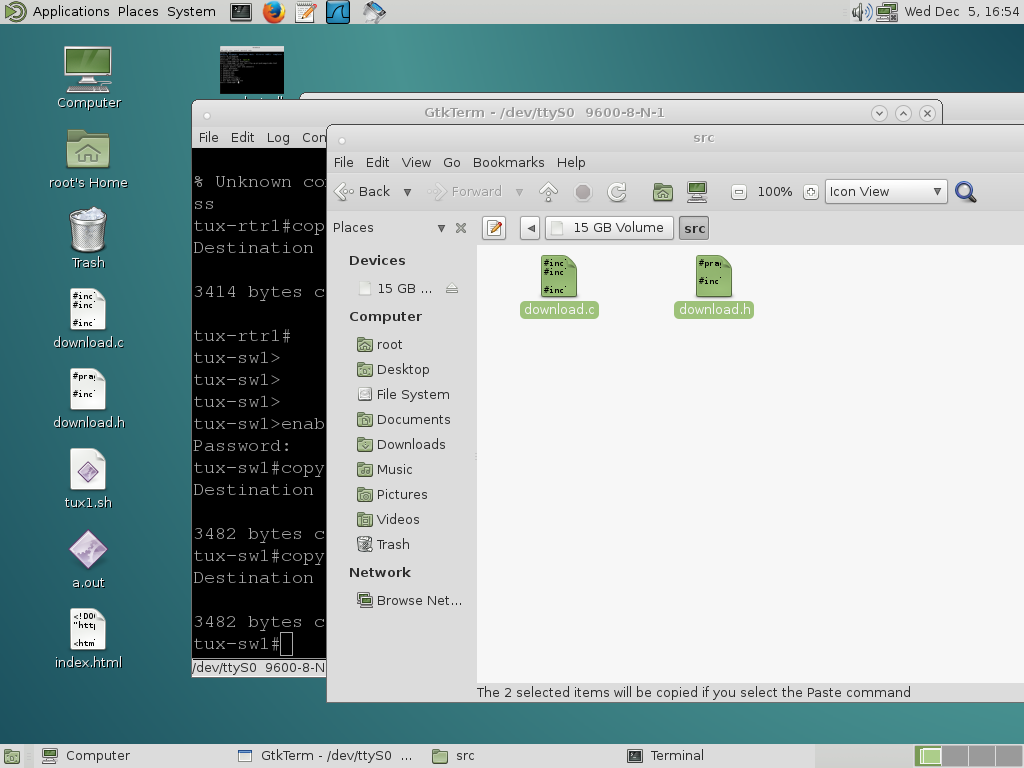
\includegraphics[width=8cm]{images/screen_dl_2.png}
\end{figure}

\begin{figure}
\end{figure}
\section{Configuração e análise de redes}
\subsection{Experiência 1 - Configurar uma rede IP}

A primeira experiência teve como objetivo ligar o \textit{tux1} ao \textit{tux4}, usando um \textit{switch}. 

\begin{enumerate}

\item O que são os pacotes ARP e para que são usados?

Os dispositivos precisam de endereços MAC (endereços físicos) para comunicarem entre si dentro da LAN, pelo que cada interface tem associada ao seu endereço IP um endereço MAC.

Quando um dispositivo (\textit{host} ou \textit{router}) pretende comunicar com outro dispositivo, apenas conhece o endereço IP com que quer comunicar, utilizando o protocolo ARP para obter o endereço MAC associado a este.

Neste protocolo são utilizados pacotes ARP (ARP \textit{request} e ARP \textit{reply}) para que um dispositivo obtenha o endereço MAC de outro dispositivo com quem pretende estabelecer uma comunicação. 

De cada vez que um dispositivo precisa obter o endereço MAC de outro dispositivo, envia um pacote de pedido (ARP \textit{request}) a todos os dispositivos, indicando o seu próprio endereço MAC e o endereço IP do dispositivo com que pretende comunicar. Como resposta, o dispositivo com o endereço IP indicado no pedido envia para o primeiro um pacote de resposta (ARP \textit{reply}) com o endereço MAC pedido, tornando-se possível a comunicação entre os dois dispositivos.

Cada dispositivo tem uma tabela ARP que guarda associações entre endereços IP e respetivos endereços MAC. Cada endereço MAC obtido por um dispositivo é guardado na sua tabela para possíveis comunicações futuras.
Em resumo, o ARP (\textit{Address Resolution Protocol}) e os pacotes ARP são utilizados para obter o endereço MAC (endereço físico/da camada de ligação) associado a um dado endereço IP (endereço IPv4 de uma interface). 


\item O que são os endereços MAC e IP dos pacotes ARP e porquê?

\textbf{O pacote ARP de pedido (APR \textit{request})} contém os endereços IP e MAC do dispositivo que faz o pedido, para que o recetor saiba qual o dispositivo que pretende obter resposta. Para além disso, contém o endereço IP do dispositivo com que se pretende estabelecer comunicação, para que este envie o seu endereço MAC como resposta. 

\textbf{O pacote ARP de resposta (APR \textit{reply})} transporta o endereço MAC solicitado até ao dispositivo que fez o pedido. 

Quando se executa o comando \mintinline{bash}{ping} do \textit{tux1} para o \textit{tux4}, o \textit{tux1} tenta comunicar com o \textit{tux4}. De acordo o protocolo descrito acima, o \textit{tux1} envia um pacote de pedido com os próprios endereços IP e MAC (172.16.10.1 e 00:21:5a:61:28:9c) e o endereço IP do \textit{tux4} (172.16.10.254), com quem pretende estabelecer conexão. Por sua vez, o \textit{tux4}, reconhecendo que o pedido é para si, envia o pacote de resposta com o seu endereço MAC (00:22:64:a6:a4:f8) para o \textit{tux1}.


\item Que pacotes gera o comando \mintinline{bash}{ping}?

O comando \mintinline{bash}{ping} começa por gerar os pacotes APR (de pedido e resposta), como referido na questão 2. De seguida são gerados pacotes do protocolo ICMP.

\item Quais são os endereços MAC e IP dos pacotes \mintinline{bash}{ping}?

Sendo o comando \mintinline{bash}{ping} executado do \textit{tux1} para o \textit{tux4}, os endereços origem correspondem aos endereços do \textit{tux1} (IP = 172.16.10.1 e MAC = 00:21:5a:61:28:9c) e os endereços destino correspondem aos endereços IP e MAC do \textit{tux4} (IP = 172.16.10.254 e MAC = 00:22:64:a6:a4:f8).

\item Como determinar se um quadro \textit{Ethernet} recebido é ARP, IP, ICMP?

O tipo de trama recebido é especificado pelo valor do \textit{Ethernet header}. O valor 0x800 indica que se trata de um IP e o valor 0x806 indica que se trata de um ARP.
Se o valor \textit{Ethernet header} for 0x0800, o valor \textit{header} do IP indica se o tipo de protocolo é ICMP (caso IP \textit{header} seja igual a 1, caso contrário está a ser usado outro protocolo).

\item Como determinar o tamanho de um quadro recebido?

O tamanho de uma frame pode ser verificado no \textit{wireshark}.

\item Qual é a interface \textit{loopback} e porque é importante?

É uma interface de rede virtual (endereço IP 127.0.0.1) que permite a um \textit{host} ou \textit{router} comunicar consigo mesmo. Trata-se de uma interface com várias utilidades, entre as quais testar se a conectividade do \textit{router} ou \textit{host} está a funcionar corretamente (ou diagnosticar problemas).
\end{enumerate}
\subsection{Experiência 2 - Implementar duas VLANs num \textit{switch}}

Na segunda experiência, começamos por criar duas LAN’s virtuais: VLAN10 e VLAN11. Posteriormente, associamos os \textit{tux1} e 4 à VLAN10 e associamos o \textit{tux2} à VLAN11.

\begin{enumerate}
\item Como configurar a \textit{vlan10}?

1) Criar uma VLAN com valor 0, usando os seguintes comandos no GTKTerm:
\begin{itemize}
    \item \mintinline{bash}{configure terminal}
    \item \mintinline{bash}{vlan y0}
    \item \mintinline{bash}{end}
\end{itemize}
2) Adicionar à VLAN criada as portas .1 e .254, que correspondem às portas do \textit{tux1} e do \textit{tux4}, respetivamente. Assim, estes \textit{tux} são ligados à VLAN0, criando-se uma sub-rede. Para tal utilizam-se os comandos:
\begin{itemize}
    \item \mintinline{bash}{configure terminal}
    \item \mintinline{bash}{interface fastethernet 0/1}  (interface fastethernet 0/254)
    \item \mintinline{bash}{switchport mode access}
    \item \mintinline{bash}{switchport access vlan y0}
    \item \mintinline{bash}{end}
\end{itemize}

\item Quantos domínios de transmissão existem? Como se pode concluir a partir dos registos?

Apesar de se executar \mintinline{bash}{ping} do \textit{tux1} para o \textit{tux4}, \mintinline{bash}{ping} do \textit{tux1} para o \textit{tux2}, e \mintinline{bash}{ping} a partir do \textit{tux2}, apenas existem 2 domínios de transmissão. O \textit{tux1} obtém resposta do \textit{tux4}, mas não obtém resposta do \textit{tux2}, assim como o \textit{tux2} não obtém resposta de qualquer outro \textit{tux} (ver figuras 2 e 3). 

Tal se justifica pelo facto de ainda não existir nenhuma ligação física entre o \textit{tux2} e os restantes \textit{tux1} e \textit{tux4}, visto que o \textit{tux2} se encontra numa sub-rede diferente da sub-rede dos restantes e vlan1 e vlan0 não têm qualquer ligação.

\end{enumerate}
\subsection{Experiência 3 - Configurar um \textit{router} em Linux}
A terceira experiência teve como propósito a configuração do \textit{tux4} como um \textit{router}, permitindo o estabelecimento de ligação entre os \textit{tux1} e \textit{tux2}, ao estabelecer uma ligação entre a VLAN01 e a VLAN11.
\begin{enumerate}
\item Que rotas existem nos \textit{tuxes}? Qual o seu significado?

O \textit{tux1} tem uma rota para a VLAN0 (172.16.y0.0) através da \textit{gateway} 172.16.y0.1 e o \textit{tux2} tem uma rota para a VLAN1 (172.16.y1.0) através da \textit{gateway} 172.16.y1.1. Estes \textit{tuxes}, juntamente com as suas rotas, representam sub-redes diferentes. Assim, o \textit{tux1} e o \textit{tux2} apenas poderão comunicar com o auxílio de um \textit{router}.

O \textit{tux4} tem duas rotas, uma para a VLAN0 pela \textit{gateway} 172.16.y0.254 e outra para a VLAN1 através da \textit{gateway} 172.16.y1.253. O \textit{tux4}, usando estas rotas, simula um \textit{router} que estabelece comunicação entre as duas sub-redes do parágrafo anterior, uma vez que estabelece comunicação entre as VLAN0 e VLAN1, permitindo, desta maneira, que o \textit{tux1} comunique com o \textit{tux2}.


\item Que informação contém uma entrada da tabela de encaminhamento?

\begin{itemize}
    \item \textit{Destination}: destino da rota
    \item \textit{Gateway}: IP da interface seguinte
    \item \textit{Interface}: eth0/etho1
\end{itemize}


\item Que mensagens ARP e endereços MAC associados são observados, e porquê?

Quando se executa \mintinline{bash}{ping} do \textit{tux1} para o \textit{tux2}, o \textit{tux1} tenta comunicar com o \textit{tux2} (comunicação possibilitada agora pelo \textit{tux4}, que simula o \textit{router}). Para tal, o \textit{tux1} começa por tentar comunicar com o \textit{tux4}, intermediário, que, por sua vez, permite que este comunique com o \textit{tux2}.

Primeiramente, o \textit{tux1} começa por enviar um pacote de pedido APR com os seus endereços IP e MAC (172.16.10.1 e 00:21:5a:61:28:9c) e o endereço IP do \textit{tux4} (172.16.10.254). O \textit{tux4} envia de volta um pacote de resposta com o seu endereço MAC (00:22:64:a6:a4:f8) para o \textit{tux1}, estabelecendo-se a comunicação entre estes.

Estando agora o \textit{tux1} ligado ao \textit{tux4}, pode enviar um pedido APR com os seus endereços e o endereço IP  172.16.11.253 (rota de ligação do \textit{tux4} com a vlan1), obtendo o endereço MAC associado ao último.

Por último, o \textit{tux1} envia finalmente o pedido com os seus endereços e o endereço do \textit{tux2} (172.16.11.1). O \textit{tux2} envia o seu endereço MAC para o \textit{tux1}, estabelecendo-se a ligação entre o \textit{tux1} e o \textit{tux2}.


\item Que pacotes ICMP são observados e porquê?

São observados tanto pacotes de pedidos como de resposta, visto que nesta experiência, ao contrário da anterior, todos os \textit{tuxes} podem comunicar entre si.

\item Quais são os endereços IP e MAC associados aos pacotes ICMP e porquê?

Os endereços associados são os endereços IP e MAC do \textit{tux} origem e os endereços IP e MAC do \textit{tux} destino.
\end{enumerate}
\subsection{Experiência 4 - Configurar um \textit{router} comercial e implementar NAT}
\begin{enumerate}
\item Como configurar uma rota estática num \textit{router} comercial?

Para fazer uma configuração de uma rota estática num \textit{router} comercial são necessárias as seguintes ligações:
\begin{itemize}
    \item Ligar porta T4 à porta do \textit{router}
    \item Ligar porta T3 à porta S0 do \textit{tux}, que deve estar ligado ao \textit{router}.
\end{itemize}
Quanto à criação da VLAN, invocam-se os seguintes comandos no GTKTerm do \textit{tux} escolhido:
\begin{itemize}
    \item \mintinline{bash}{configure terminal}
    \item \mintinline{bash}{ip route [IP da porta de destino] [máscara] [IP gateway]}
    \item \mintinline{bash}{exit}
\end{itemize}


\item Quais são os caminhos seguidos pelos pacotes nas experiências feitas e porquê?

Nas experiências, os pacotes seguem ou rotas existentes, ou a rota \textit{default}.
Se uma rota já existir definida, os pacotes seguem essa mesma, em caso contrário, os pacotes vão até ao \textit{router}, este dá o sinal de que o \textit{tux4} existe e que devem ser enviados através do mesmo.

\item Como configurar NAT num \textit{router} comercial?

A configuração do NAT foi feita seguindo o guião da experiência 4, através do GTKTerm, apresentados em seguida:
\begin{itemize}
    \item  \mintinline{bash}{conf t}
    \item  \mintinline{bash}{interface gigabitethernet 0/0 *}
    \item  \mintinline{bash}{ip address 172.16.y1.254 255.255.255.0}
    \item  \mintinline{bash}{no shutdown}
    \item  \mintinline{bash}{ip nat inside}
    \item  \mintinline{bash}{exit}
    \item  \mintinline{bash}{interface gigabitethernet 0/1*}
    \item  \mintinline{bash}{ip address 172.16.1.y9 255.255.255.0}
    \item  \mintinline{bash}{no shutdown}
    \item  \mintinline{bash}{ip nat outside}
    \item  \mintinline{bash}{exit}
    \item  \mintinline{bash}{ip nat pool ovrld 172.16.1.y9 172.16.1.y9 prefix 24}
    \item  \mintinline{bash}{ip nat inside source list 1 pool ovrld overload}
    \item  \mintinline{bash}{access-list 1 permit 172.16.y0.0 0.0.0.7}
    \item  \mintinline{bash}{access-list 1 permit 172.16.y1.0 0.0.0.7}
    \item  \mintinline{bash}{ip route 0.0.0.0 0.0.0.0 172.16.1.254}
    \item  \mintinline{bash}{ip route 172.16.y0.0 255.255.255.0 172.16.y1.253}
    \item  \mintinline{bash}{end}
\end{itemize}


\item O que faz NAT?

O NAT (\textit{Network Adress Translation}) permite que os computadores de uma rede interna, como a que foi criada no desenvolvimento deste projeto, possa ter acesso à rede exterior, sendo que fora da sua rede, possa ser reconhecida através de um IP único, representante de todos os dispositivos que contém.
Isto é possivel porque o NAT opera num \textit{router} que conecta duas redes. Faz depois a tradução dos IPs privados para IPs legais e permite o encaminhamento de pacotes para a rede exterior.
Funciona ainda como medida de segurança e é implementado com frequência em ambientes de acesso remoto.

\end{enumerate}
\subsection{Experiência 5 - DNS}
\begin{enumerate}
\item Como configurar o servico DNS num anfitrião?

O serviço de DNS é configurado no ficheiro localizado em \mintinline{bash}{vi/etc/resolv.conf} no anfitrião \textit{tux} desejado.
A configuração é feita através de dois comandos que serão apresentados em seguida. Estes comandos representam o nome do servidor DNS e o respetivo endereço IP. Depois de executados permitem a conexão à internet.
\begin{itemize}
    \item \mintinline{bash}{search netlab.fe.up.pt}
    \item \mintinline{bash}{nameserver 172.16.1.1}
\end{itemize}

\item Que pacotes são trocados por DNS e que informação é transportada?

O \textit{host} envia para o servidor um pacote com o \textit{hostname} em questão, esperando que seja retornado o seu endereço de IP.
O servidor responde em seguida com um pacote contendo o endereço IP do \textit{hostname} em questão.

\end{enumerate}
\subsection{Experiência 6 - Conexões TCP}
\begin{enumerate}
\item Quantas conexões TCP são abertas pela aplicação FTP?

São abertas 2 conexões. A primeira, para enviar os comandos FTP ao servidor e receber a respetiva resposta.
A segunda para a receção de dados enviados pelo servidor e respetiva resposta do cliente.

\item Em que conexão é transportada a informação de controlo FTP?

Na conexão TCP responsável pela troca de comandos.
\item Quais são as fases de uma conexão FTP?

Uma conexão FTP tem as 3 seguintes fases:
\begin{itemize}
    \item Estabelecimento da conexão
    \item Troca de dados
    \item Encerramento da conexão
\end{itemize}


\item Como funciona o mecanismo ARQ TCP? Quais são os campos TCP relevantes? Que informação relevante pode ser observada nos
registos?

O mecanismo ARQ TCP funciona com o método da janela deslizante, ou seja, com o controlo de erros na transmissão de dados. 
Este controlo de erros é feito através de \textit{acknowledgment numbers}, enviados pelo recetor e que indicam se a trama foi recebida corretamente, \textit{window size} indicando a gama dos pacotes recebidos e o número do pacote a ser enviado, o \textit{sequence number}.

\item Como funciona o mecanismo de congestionamento de controlo TCP? Quais são os campos relevantes? Como é que
a taxa de transferência da conexão de dados evoluiu ao longo do tempo? Está de acordo com o mecanismo de congestionamento de controlo TCP?

O TCP contém uma janela de congestão. Isto é, uma estimativa do número de octetos que a rede consegue encaminhar, não enviando assim mais octetos que o mínimo da janela definida.
O fluxo de dados de conexão do nosso projeto está de acordo com o mecanismo de controlo de congestão, uma vez que sempre que o congestionamento de rede aumentava, o bitrate diminuia.

\item A taxa de transferência de uma conexão de dados TCP é perturbada pelo aparecimento de uma segunda conexão TCP? Como?

Sim. O aparecimento de uma segunda conexão TCP pode levar a uma queda na taxa de transmissão. Esta é distribuida de forma igual para cada ligação e por isso é lógico que com o aparecimento de uma nova conexão, a taxa de transferência seja reduzida.

\end{enumerate}
\section{Conclusão}
Consideramos que, com o desenvolvimento deste projeto, fomos capazes de cumprir, com sucesso, os objetivos inicialmente propostos.  Acrescentamos ainda que este trabalho permitiu a exploração e assimilação de uma série de conceitos, fundamentais para o conhecimento e domínio das redes de computadores.  
\begin{thebibliography}{1}
    \bibitem{rfc959} 
    File Transfer Protocol Standard,
    \\\texttt{https://tools.ietf.org/html/rfc959}
\end{thebibliography}
\pagebreak

\section{Anexos}
\subsection{Código da aplicação \textit{download}}
\textbf{download.h}
\begin{minted}{c}
#pragma once

#include <stdbool.h>

#define MAX_BUF_SIZE 100
#define MAX_REPLY_SIZE 400
#define SOCKET_BUF_SIZE 1000
#define REPLY_CODE_SIZE 3
#define SERVER_PORT 21

typedef struct
{
    char serverName[MAX_BUF_SIZE];
    char filePath[MAX_BUF_SIZE];
    char fileName[MAX_BUF_SIZE];
    char user[MAX_BUF_SIZE];
    char pass[MAX_BUF_SIZE];
} info_t;

typedef enum
{
    READ_CODE,
    READ_LINE,
    READ_MULT_LINE,
    WAIT_FOR_PORT,
    FIRST_PORT_BYTE,
    SECOND_PORT_BYTE,
    END
} state_t;

typedef enum
{
    POSITIVE_PRE = 1,
    POSITIVE_INT,
    POSITIVE_COMP,
    TRANS_NEGATIVE_COMP,
    PERM_NEGATIVE_COMP
} reply_type_t;

/**
 * @brief Prints a message that shows how to run the program.
 * 
 * @param argv array of arguments passed from the command line
 * 
 * @return always return 1
 */
int usage(char *argv[]);

/**
 * @brief Parses the argument passed to the program, retrieving user information.
 * 
 * @param argument argument from the command line, supposedly an FTP link
 * @param info structure that holds user and server info
 * 
 * @return true if argument was successfully read, false otherwise 
 */
bool parseArgument(char *argument, info_t *info);

/**
 * @brief Gets a server ip from a host name
 * 
 * @param name host name
 * 
 * @return server ip 
 */
char *getServerIp(const char* name);

/**
 * @brief Creates a TCP socket, returning its respective file descriptor.
 * 
 * @param server_ip 
 * @param server_port 
 * 
 * @return socket's file descriptor 
 */
int createSocketTCP(char *server_ip, int server_port);

/**
 * @brief Reads the server reply to an FTP command, returning it through the reply argument.
 * 
 * @param socketFd socket's file descriptor
 * @param reply numeric descriptor of the server reply
 */
void readServerReply(int socketFd, char *reply);

/**
 * @brief Gets the server port after the program issues pasv command.
 * 
 * @param socketFd socket's file descriptor
 * 
 * @return the server port
 */
int getServerPort(int socketFd);

/**
 * @brief Sends and FTP command along with its argument (if applicable) and reads the server reply.
 * 
 * 
 * @param socketFd socket's file descriptor
 * @param command FTP command
 * @param argument command's argument, if any
 * 
 * @return 0 for POSITIVE_INT, 1 for POSITIVE_COMP and -1 for PERM_NEGATIVE_COMP
 */
int sendCommand(int socketFd, char *command, char *argument);

/**
 * @brief Called after sending RETR command, reads data from the socket and creates a local file.
 * 
 * @param fd second socket's file descriptor
 * @param filename name of the file to be retrieved
 */
void createFile(int fd, char *filename);
\end{minted}

\textbf{download.c}
\begin{minted}{C}
#include <arpa/inet.h>
#include <netinet/in.h>

#include <sys/socket.h>
#include <sys/types.h>

#include <ctype.h>
#include <errno.h>
#include <netdb.h>
#include <signal.h>
#include <stdio.h>
#include <stdlib.h>
#include <string.h>
#include <strings.h>
#include <unistd.h>
    
#include "download.h"

int usage(char *argv[])
{
    printf("Usage: %s ftp://[<user>:<password>@]<host>/<url-path>\n", argv[0]);
    return 1;
}

bool parseArgument(char *argument, info_t *info)
{
    char *sep;
    char* lastSep;
    int index1 = 6, index2;

    if (strncmp("ftp://", argument, 6) != 0)
        return false;

    if ((sep = strchr(argument + 6, ':')) != NULL)
    {
        int index;

        index = (int)(sep - argument);
        strncpy(info->user, argument + 6, index - 6);
        info->user[index - 6] = '\0';

        if ((sep = strchr(argument, '@')) == NULL)
            return false;

        int new_index = (int)(sep - argument);
        index++;
        strncpy(info->pass, argument + index, new_index - index);
        info->pass[new_index - index] = '\0';

        index1 = ++new_index;
    }
    else if ((sep = strchr(argument, '@')) != NULL)
        return false;
    else
        strncpy(info->user, "placeholder", 11);

    if ((sep = strchr(argument + 6, '/')) == NULL)
        return false;

    index2 = (int)(sep - argument);

    strncpy(info->serverName, argument + index1, index2 - index1);
    info->serverName[index2 - index1] = '\0';
    index2++;
    strncpy(info->filePath, argument + index2, strlen(argument) - index2);
    info->filePath[strlen(argument) - index2] = '\0';

    lastSep = strrchr(argument, '/');
    strcpy(info->fileName, lastSep + 1);
    info->fileName[strlen(lastSep)] = '\0';

    return true;
}

char *getServerIp(const char* name) 
{
    struct hostent *h;

    if ((h = gethostbyname(name)) == NULL) 
    {
        herror("gethostbyname");
        exit(1);
    }

    return inet_ntoa(*((struct in_addr *)h->h_addr_list[0]));
}

int createSocketTCP(char *server_ip, int server_port)
{
    int socketFd;
    struct sockaddr_in server_addr;

    /*server address handling*/
    bzero((char *)&server_addr, sizeof(server_addr));
    server_addr.sin_family = AF_INET;
    server_addr.sin_addr.s_addr =
        inet_addr(server_ip); /*32 bit Internet address network byte ordered*/
    server_addr.sin_port =
        htons(server_port); /*server TCP port must be network byte ordered */

    /*open an TCP socket*/
    if ((socketFd = socket(AF_INET, SOCK_STREAM, 0)) < 0)
    {
        perror("socket()");
        exit(0);
    }

    /*connect to the server*/
    if (connect(socketFd, (struct sockaddr *)&server_addr, sizeof(server_addr)) <
        0)
    {
        perror("connect()");
        exit(0);
    }

    return socketFd;
}

void readServerReply(int socketFd, char *reply)
{
    char c;
    int res = 0, i = 0;
    state_t state = READ_CODE;

    while (state != END)
    {
        if ((res = read(socketFd, &c, 1)) <= 0)
            continue;

        switch (state)
        {
        case READ_CODE:
            if (c == ' ')
            {
                state = READ_LINE;
                i = 0;
            }
            else if (c == '-')
            {
                state = READ_MULT_LINE;
                i = 0;
            }
            else if (isdigit(c))
            {
                reply[i++] = c;
            }
            break;
        case READ_LINE:
            if (c == '\n')
                state = END;
            break;
        case READ_MULT_LINE:
            if (c == reply[i])
            {
                i++;
            }
            else if (i == 3 && c == ' ')
            {
                state = READ_LINE;
            }
            break;
        case END:
            break;
        default:
            break;
        }
    }
}

int getServerPort(int socketFd)
{
    int res = 0;
    state_t state = WAIT_FOR_PORT;
    char c;
    char first_byte[4], second_byte[4];
    int numCommas = 0, i = 0;

    while (state != END)
    {
        if ((res = read(socketFd, &c, 1)) <= 0)
            continue;

        switch (state)
        {
        case READ_CODE:
            if (c == ' ')
            {
                if (i != 3)
                {
                    printf(" > Error receiving response code\n");
                    return -1;
                }
                i = 0;
                state = WAIT_FOR_PORT;
            }
            else
            {
                i++;
            }
            break;
            break;
        case WAIT_FOR_PORT:
            if (c == ',')
                numCommas++;

            if (numCommas == 4)
                state = FIRST_PORT_BYTE;
            break;
        case FIRST_PORT_BYTE:
            if (c == ',')
            {
                state = SECOND_PORT_BYTE;
                i = 0;
            }
            else
            {
                first_byte[i++] = c;
            }
            break;
        case SECOND_PORT_BYTE:
            if (c == ')')
                state = END;
            else
            {
                second_byte[i++] = c;
            }
            break;
        case END:
            break;
        default:
            break;
        }
    }

    return atoi(first_byte) * 256 + atoi(second_byte);
}

int sendCommand(int socketFd, char *command, char *argument)
{
    char reply[REPLY_CODE_SIZE];
    reply_type_t type;

    write(socketFd, command, strlen(command));
    if (argument != NULL)
        write(socketFd, argument, strlen(argument));
    write(socketFd, "\n", 1);

    while (true)
    {
        readServerReply(socketFd, reply);

        type = reply[0] - '0';

        switch (type)
        {
        case POSITIVE_PRE:
            break;
        case POSITIVE_INT:
            return 0;
        case POSITIVE_COMP:
            return 1;
        case TRANS_NEGATIVE_COMP:
            write(socketFd, command, strlen(command));
            if (argument != NULL)
                write(socketFd, argument, strlen(argument));
            write(socketFd, "\n", 1);
            break;
        case PERM_NEGATIVE_COMP:
            close(socketFd);
            return -1;
        default:
            break;
        }
    }
}

void createFile(int fd, char *filename)
{
    FILE *file = fopen(filename, "wb+");

    char fileData[SOCKET_BUF_SIZE];
    int nbytes;
    while ((nbytes = read(fd, fileData, SOCKET_BUF_SIZE)) > 0)
    {
        nbytes = fwrite(fileData, nbytes, 1, file);
    }

    fclose(file);
}

int main(int argc, char *argv[])
{
    info_t info;
    char *server_ip;
    char reply[MAX_REPLY_SIZE];
    int fd1, fd2, res, port;

    if (argc != 2 || !parseArgument(argv[1], &info))
        return usage(argv);

    server_ip = getServerIp(info.serverName);

    fd1 = createSocketTCP(server_ip, SERVER_PORT);
    readServerReply(fd1, reply);

    if (reply[0] == '2')
        printf(" > Connection established!\n");
    else
    {
        printf(" > Couldn't connect! Exiting.\n");
        exit(1);
    }

    if(strncmp(info.user, "placeholder", 11) == 0){
        printf(" > Please specify user and password.\n");
        printf(" > User: ");
        scanf("%s", info.user);
        printf(" > Password: ");
        scanf("%s", info.pass);
    }

    printf(" > Sending user\n");
    res = sendCommand(fd1, "user ", info.user);

    if (res == 0 || res == 1)
    {
        printf(" > Sending pass\n");
        res = sendCommand(fd1, "pass ", info.pass);
    }
    else
    {
        printf(" > Error sending username! Exiting.\n");
        exit(1);
    }

    write(fd1, "pasv\n", 5);
    port = getServerPort(fd1);

    fd2 = createSocketTCP(server_ip, port);

    printf(" > Sending retr\n");
    res = sendCommand(fd1, "retr ", info.filePath);

    if (res == 0)
    {
        printf(" > Downloading file...\n");
        createFile(fd2, info.fileName);
    }

    printf(" > Quiting connection\n");
    write(fd1, "quit\n", 5);

    close(fd1);
    close(fd2);

    printf(" > All done! Exiting now\n");
    return 0;
}    
\end{minted}
\subsection{Comandos de configuração}
De forma a facilitar a configuração dos \textit{tuxes}, foram desenvolvidos os seguintes \textit{bash scripts}.

\textbf{tux1.sh}
\begin{minted}{bash}
#!/bin/bash

if [ $# != 1 ] || [ $1 -lt 1 ] || [ $1 -gt 6 ]; then
    echo "Usage: $0 <stand>"
    exit 1
fi

ip1="172.16.$10.1/24"
ip2="172.16.$11.0/24"
ip3="172.16.$10.254"

ifconfig eth0 up
ifconfig eth0 $ip1
route add -net $ip2 gw $ip3
route add default gw $ip3
\end{minted}

\textbf{tux2.sh}
\begin{minted}{bash}
#!/bin/bash

if [ $# != 1 ] || [ $1 -lt 1 ] || [ $1 -gt 6 ]; then
    echo "Usage: $0 <stand>"
    exit 1
fi

ip1="172.16.$11.1/24"
ip2="172.16.$10.0/24"
ip3="172.16.$11.253"
ip4="172.16.$11.254"

ifconfig eth0 up
ifconfig eth0 $ip1
route add -net $ip2 gw $ip3
route add default gw $ip4
\end{minted}

\textbf{tux4.sh}
\begin{minted}{bash}
#!/bin/bash

if [ $# != 1 ] || [ $1 -lt 1 ] || [ $1 -gt 6 ]; then
    echo "Usage: $0 <stand>"
    exit 1
fi

ip1="172.16.$10.254/24"
ip2="172.16.$11.253/24"
ip3="172.16.$11.254"

ifconfig eth0 up
ifconfig eth0 $ip1
ifconfig eth1 up
ifconfig eth1 $ip2
echo 1 > /proc/sys/net/ipv4/ip_forward
echo 0 > /proc/sys/net/ipv4/icmp_echo_ignore_broadcasts
route add default gw $ip3
\end{minted}
\subsection{\textit{Logs} registados}
\begin{figure}[H]
    \centering
    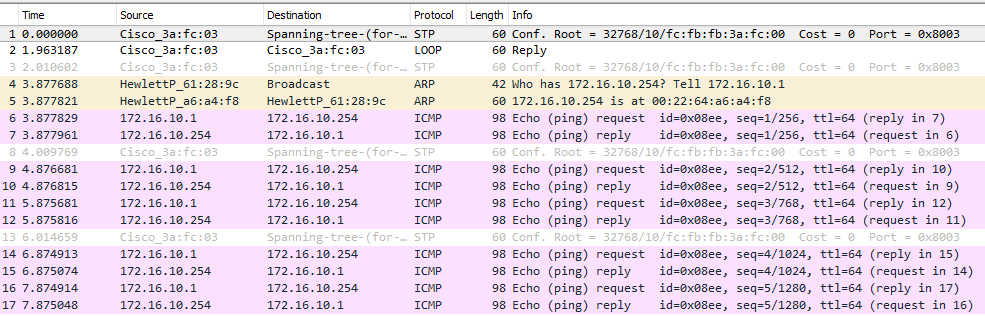
\includegraphics[scale=0.5]{images/exp1.PNG}
    \caption{Experiência 1 (ping do tux1 para tux4)}
\end{figure}
\begin{figure}[H]
    \centering
    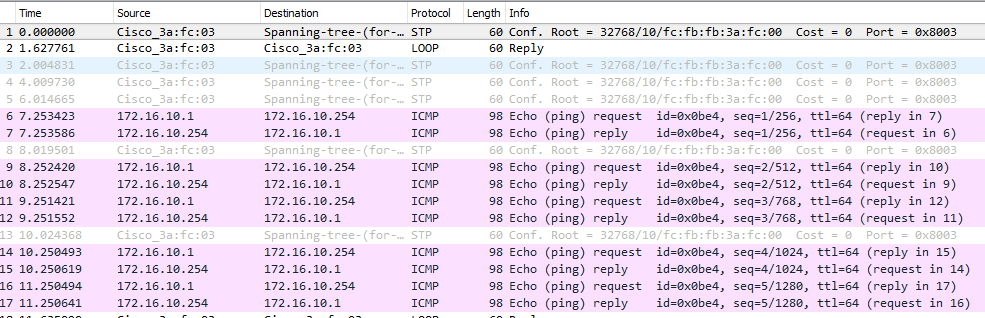
\includegraphics[scale=0.5]{images/exp2_1_4.PNG}
    \caption{Experiência 2 (ping do tux1 para o tux4)}
\end{figure}
\begin{figure}[H]
    \centering
    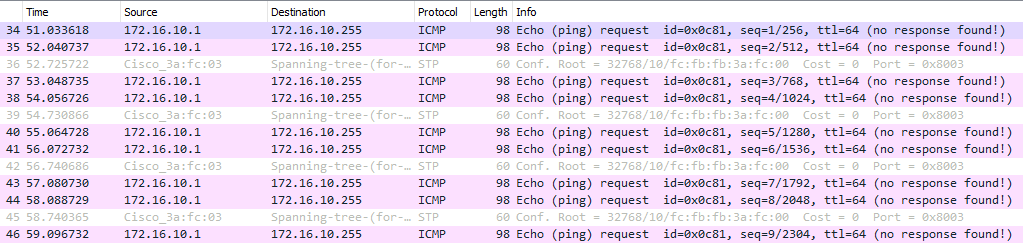
\includegraphics[scale=0.5]{images/exp2_1_2.PNG}
    \caption{Experiência 2 (ping do tux1 para o tux2)}
\end{figure}
\begin{figure}[H]
    \centering
    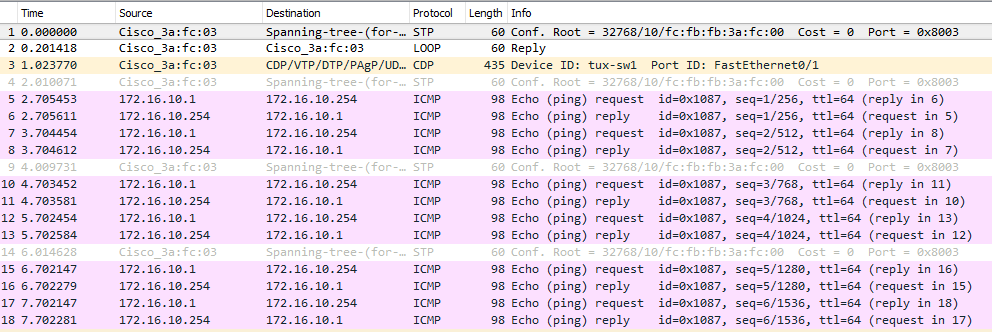
\includegraphics[scale=0.5]{images/exp3_part1.PNG}
    \caption{Experiência 3 (ping do tux1 para o tux2, part1)}
\end{figure}
\begin{figure}[H]
    \centering
    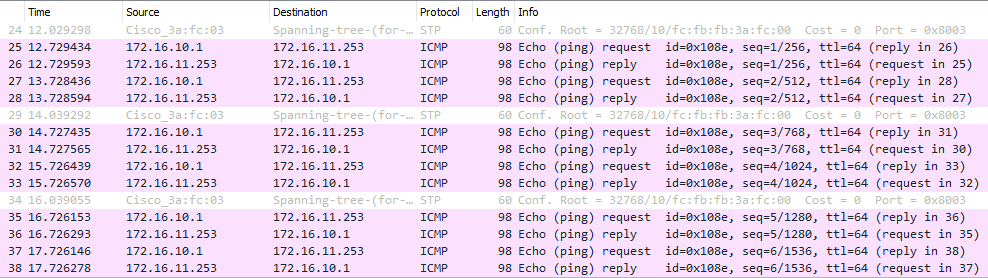
\includegraphics[scale=0.5]{images/exp3_part2.PNG}
    \caption{Experiência 3 (ping do tux1 para o tux2, part2)}
\end{figure}
\begin{figure}[H]
    \centering
    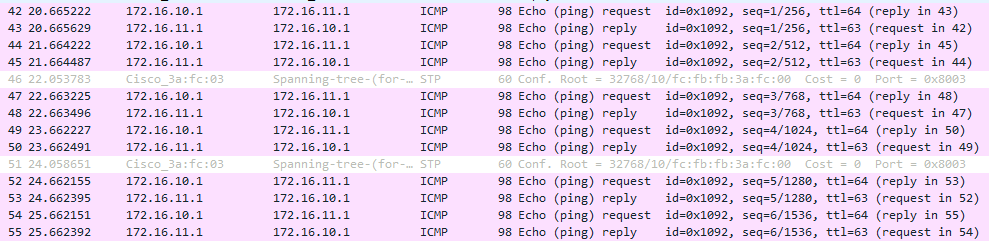
\includegraphics[scale=0.5]{images/exp3_part3.PNG}
    \caption{Experiência 3 (ping do tux1 para o tux2, part3)}
\end{figure}

\end{document}